\documentclass[aspectratio=169]{beamer}
\usepackage{graphicx}
\usepackage{amsmath}
\usepackage{amssymb}
\usepackage{booktabs}
\usepackage{xcolor}
\usepackage{tikz}
\usepackage{pgfplots}
\usepackage{pifont}

% Theme
\usetheme{Madrid}
\usecolortheme{beaver}

% Colors
\definecolor{primaryblue}{RGB}{0,102,204}
\definecolor{successgreen}{RGB}{40,167,69}
\definecolor{warningorange}{RGB}{255,193,7}

% Title page information
\title{Geometrical Reconstruction using Acoustic Tactile Sensing}
\author{Georg Wolnik}
\date{November 11, 2025}
\begin{document}

% Title slide
\begin{frame}
\titlepage
\end{frame}

% Slide 1: Overview
\begin{frame}{Overview}
\textbf{Goal:} How can we maximize the use of acoustic signals for geometrical reconstruciton

\vspace{1em}
\textbf{Questions:}
\begin{itemize}
    \item Can we replicate the classification results with our current setup?
    \item What information specifically can we extract from the acoustic signals?
    \item What features are most important?
\end{itemize}
\end{frame}

% Slide 2: Data and Features
\begin{frame}{Data and Features}
\textbf{Dataset:}
\begin{itemize}
    \item 4 experimental batches, 650 total samples, 50 samples per class
    \item 2-second broadband chirp signals (20Hz-20kHz)
\end{itemize}

\vspace{1em}
\textbf{Data:}
\begin{itemize}
    \item Contact position classification (tip/middle/base/no contact) (Batch 1+2)
    \item Edge detection (contact/edge/no edge) (Batch 2)
    \item Fine feature detection (paper clip present/absent) (Batch 3)
\end{itemize}

\vspace{1em}
\textbf{Features Extracted:}
\begin{itemize}
    \item 38 acoustic features (spectral, temporal, frequency domain)
    \item 15 impulse response features (transfer function characteristics)
    \item Total: 53 features per sample
\end{itemize}
\end{frame}

% Slide 3: Acoustic Features - Spectral
\begin{frame}{Acoustic Features: Spectral (13)}
\footnotesize
\begin{itemize}
    \item \texttt{spectral\_centroid} - Center of mass of spectrum
    \item \texttt{spectral\_bandwidth} - Spread around centroid
    \item \texttt{spectral\_rolloff} - 85\% energy frequency
    \item \texttt{spectral\_flux} - Spectral change rate
    \item \texttt{spectral\_flatness} - Noise vs tone measure
    \item \texttt{spectral\_contrast} - Peak-to-valley differences
\end{itemize}

\vspace{0.5em}
\textbf{Temporal Features (8):}
\begin{itemize}
    \item \texttt{zero\_crossing\_rate} - Signal noisiness
    \item \texttt{rms\_energy} - Signal energy
    \item \texttt{envelope\_features} - Amplitude properties
\end{itemize}

\textbf{Reference:} Zöller et al. (2020) \cite{zoeller2020active}
\end{frame}

% Slide 4: Acoustic Features - MFCC and High-Freq
\begin{frame}{Acoustic Features: MFCC and High-Frequency}
\footnotesize
\textbf{MFCC Features (12):}
\begin{itemize}
    \item \texttt{mfcc\_0 to mfcc\_11} - Mel-scale cepstral coefficients
    \item Perceptually relevant spectral representation
    \item Capture timbre and spectral envelope
\end{itemize}

\vspace{0.5em}
\textbf{High-Frequency Features (5):}
\begin{itemize}
    \item \texttt{ultra\_high\_energy\_ratio} - Energy >8kHz
    \item \texttt{ultra\_high\_ratio} - High-freq to total energy
    \item \texttt{high\_freq\_content} - High-frequency measures
\end{itemize}

\textbf{Why These Features?}
\begin{itemize}
    \item Standard in audio signal processing
    \item Sensitive to geometric and material changes
\end{itemize}

\textbf{Reference:} Wall et al. (2022) \cite{wall2022passive}
\end{frame}

% Slide 5: Impulse Response Features - Magnitude
\begin{frame}{Impulse Response Features: Magnitude (8)}
\footnotesize
\begin{itemize}
    \item \texttt{freq\_response\_centroid} - Transfer function center of mass
    \item \texttt{freq\_response\_bandwidth} - Transfer function spread
    \item \texttt{freq\_response\_skewness} - Transfer function asymmetry
    \item \texttt{freq\_response\_kurtosis} - Transfer function peakedness
    \item \texttt{resonance\_peak\_magnitude} - Strongest resonance height
    \item \texttt{resonance\_peak\_frequency} - Strongest resonance frequency
    \item \texttt{resonance\_bandwidth} - Resonance peak width
    \item \texttt{resonance\_skewness} - Resonance distribution asymmetry
\end{itemize}

\textbf{Reference:} Zöller et al. (2020) \cite{zoeller2020active}
\end{frame}

% Slide 6: Impulse Response Features - Decay
\begin{frame}{Impulse Response Features: Decay and Damping (7)}
\footnotesize
\begin{itemize}
    \item \texttt{decay\_amplitude} - Amplitude decay rate
    \item \texttt{decay\_time} - Exponential decay time constant
    \item \texttt{damping\_ratio} - System damping measure
    \item \texttt{quality\_factor} - Resonance sharpness (Q-factor)
\end{itemize}

\vspace{0.5em}
\textbf{Why Impulse Response Features?}
\begin{itemize}
    \item True system characterization independent of input
    \item Captures physical properties: resonances, damping, stiffness
    \item Complements traditional acoustic features
\end{itemize}

\textbf{Reference:} Rompf (2019) \cite{rompf2019thesis}
\end{frame}

% Slide 7: Dimensionality Reduction Methods
\begin{frame}{Dimensionality Reduction: PCA and t-SNE}
\footnotesize
\begin{columns}
\column{0.48\textwidth}
\textbf{Principal Component Analysis (PCA):}
\begin{itemize}
    \item Linear technique finding maximum variance directions
    \item Projects high-dimensional data to lower dimensions
    \item Preserves global structure and distances
    \item Based on eigenvalue decomposition of covariance matrix
\end{itemize}

\column{0.48\textwidth}
\textbf{t-Distributed Stochastic Neighbor Embedding (t-SNE):}
\begin{itemize}
    \item Nonlinear technique preserving local neighborhoods
    \item Converts similarities to probability distributions
    \item Minimizes KL divergence between distributions
    \item Excellent for visualizing high-dimensional clusters
\end{itemize}
\end{columns}

\vspace{2em}
\textbf{Purpose:} Reduce 53D feature space to 2D for visualization and assess class separability
\end{frame}

% Slide 8: PCA and t-SNE Results
\begin{frame}{PCA and t-SNE: Class Discrimination}
\footnotesize
\textbf{Visualization Results:}
\begin{itemize}
    \item PCA (left): Shows linear separability of classes
    \item t-SNE (right): Reveals nonlinear cluster structure
    \item Clear class separation indicates discriminative features
\end{itemize}

\vspace{0.5em}
\includegraphics[width=\textwidth, height=0.6\textheight]{soft_finger_batch_2_method_comparison.png}
\end{frame}

% Slide 9: Transfer Function - Input Signal
\begin{frame}{Transfer Function: The Input Sweep}
\begin{columns}
\column{0.6\textwidth}
\footnotesize
\textbf{What We Send: Broadband Chirp Signal}
\begin{itemize}
    \item Linear frequency sweep from 20Hz to 20kHz
    \item 2-second duration for good frequency resolution
    \item Known, controlled input signal
    \item Excites all frequencies of interest
\end{itemize}

\vspace{0.5em}
\textbf{Signal Properties:}
\begin{itemize}
    \item Constant amplitude across frequencies
    \item Linear frequency increase over time
    \item Designed to characterize system response
\end{itemize}
\column{0.35\textwidth}
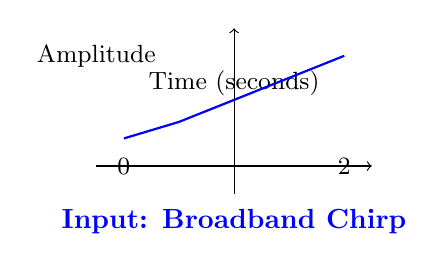
\begin{tikzpicture}[scale=0.7]
    % Conceptual sweep signal
    \node at (0,1.5) {\small Time (seconds)};
    \node at (-2,0) {\small 0};
    \node at (2,0) {\small 2};
    \draw[->] (-2.5,0) -- (2.5,0);
    \draw[->] (0,-0.5) -- (0,2.5);
    
    \node at (-2.5,2) {\small Amplitude};
    
    % Sweep line
    \draw[thick, blue] (-2,0.5) -- (-1,0.8) -- (0,1.2) -- (1,1.6) -- (2,2.0);
    
    \node[blue] at (0,-1) {\textbf{Input: Broadband Chirp}};
\end{tikzpicture}
\end{columns}
\end{frame}

% Slide 10: Transfer Function - Received Signal
\begin{frame}{Transfer Function: What We Receive}
\begin{columns}
\column{0.6\textwidth}
\footnotesize
\textbf{What We Record: Modified Response}
\begin{itemize}
    \item Microphone captures the acoustic response
    \item Signal is modified by finger-object interaction
    \item Same duration as input signal (2 seconds)
\end{itemize}

\vspace{2em}
\textbf{Key Observation:}
\begin{itemize}
    \item Different contact conditions produce different responses
    \item More information (features) can be used for classification
\end{itemize}
\column{0.35\textwidth}
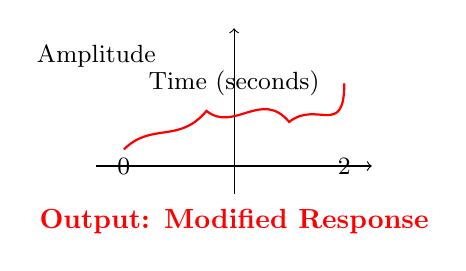
\begin{tikzpicture}[scale=0.7]
    % Conceptual received signal
    \node at (0,1.5) {\small Time (seconds)};
    \node at (-2,0) {\small 0};
    \node at (2,0) {\small 2};
    \draw[->] (-2.5,0) -- (2.5,0);
    \draw[->] (0,-0.5) -- (0,2.5);
    
    \node at (-2.5,2) {\small Amplitude};
    
    % Modified response line (more complex)
    \draw[thick, red] (-2,0.3) .. controls (-1.5,0.8) and (-1,0.4) .. (-0.5,1.0) .. controls (0,0.6) and (0.5,1.4) .. (1,0.8) .. controls (1.5,1.2) and (2,0.5) .. (2,1.5);
    
    \node[red] at (0,-1) {\textbf{Output: Modified Response}};
\end{tikzpicture}
\end{columns}
\end{frame}

% Slide 11: Transfer Function - Calculation
\begin{frame}{Transfer Function: Deconvolution Process}
\footnotesize
\textbf{Computing the Transfer Function:}

\vspace{0.3em}
\textbf{1. Fourier Transform Both Signals:}
\begin{itemize}
    \item X(f) = FFT[input sweep]
    \item Y(f) = FFT[received response]
\end{itemize}

\vspace{0.3em}
\textbf{2. Deconvolution:}
\begin{itemize}
    \item H(f) = Y(f) / X(f)
    \item Normalize by input spectrum
\end{itemize}

\vspace{0.3em}
\textbf{3. Result:}
\begin{itemize}
    \item Transfer function H(f) shows how the system modifies each frequency
    \item Magnitude H(f) reveals resonances and damping
\end{itemize}

\begin{alertblock}{Key Advantage}
Transfer function is independent of the input signal - it characterizes the acoustic system itself
\end{alertblock}
\end{frame}


% Slide 13: Transfer Function - Additional Features
\begin{frame}{Transfer Function: Additional Features}
\footnotesize
\textbf{With Transfer Function, We Now Have Access To:}

\vspace{0.3em}
\textbf{15 New Impulse Response Features:}
\begin{itemize}
    \item Resonance characteristics (frequency, magnitude, bandwidth)
    \item System damping properties (Q-factor, decay rates)
    \item Frequency response statistics (centroid, bandwidth, skewness)
    \item Properties independent of the specific input signal
\end{itemize}

\vspace{0.3em}
\textbf{Why This Matters:}
\begin{itemize}
    \item Traditional acoustic features depend on input signal design
    \item Impulse response features characterize the physical system
    \item Provides complementary information to acoustic features
\end{itemize}

\begin{alertblock}{Result}
Combined acoustic (38) + impulse response (15) = 53 total features for training
\end{alertblock}

\textbf{Reference:} Zöller et al. (2020) \cite{zoeller2020active}, Rompf (2019) \cite{rompf2019thesis}
\end{frame}

% Slide 14: Saliency Analysis - Input and Method
\begin{frame}{Saliency Analysis: Input and How It Works}
\footnotesize
\textbf{Input to Saliency Analysis:}
\begin{itemize}
    \item Complete dataset: 650 samples × 53 features each
    \item Includes both acoustic (38) and impulse response (15) features
\end{itemize}

\vspace{0.5em}
\textbf{How Saliency Analysis Works:}
\begin{itemize}
    \item Train neural network classifier on all 53 features
    \item For each feature, compute how much it affects the network's predictions
    \item Use backpropagation to calculate gradients w.r.t. input features
    \item Higher gradient magnitude = more important feature
\end{itemize}

\vspace{0.5em}
\textbf{Method Details:}
\begin{itemize}
    \item TensorFlow/Keras implementation
    \item Multiple hidden layers for complex feature interactions
\end{itemize}
\end{frame}

% Slide 15: Saliency Analysis - Results and Interpretation
\begin{frame}{Saliency Analysis: Results and What They Mean}
\footnotesize
\begin{columns}
\column{0.55\textwidth}
\textbf{Top 6 Most Important Features:}
\begin{enumerate}
    \item \texttt{spectral\_bandwidth} - Frequency spread (acoustic)
    \item \texttt{resonance\_skewness} - Resonance asymmetry (impulse)
    \item \texttt{freq\_response\_centroid} - Response center (impulse)
    \item \texttt{ultra\_high\_energy\_ratio} - High-freq energy (acoustic)
    \item \texttt{decay\_amplitude} - Signal decay rate (impulse)
    \item \texttt{ultra\_high\_ratio} - High-freq ratio (acoustic)
\end{enumerate}

\vspace{0.5em}
\textbf{Key Results:}
\begin{itemize}
    \item 3 of top 6 features are impulse response derived
    \item Mixed importance between acoustic and impulse response features
\end{itemize}

\column{0.4\textwidth}
\includegraphics[width=\textwidth, height=0.7\textheight]{soft_finger_batch_2_saliency_analysis.png}
\end{columns}
\end{frame}

% Slide 16: Saliency Analysis - Insights
\begin{frame}{Saliency Analysis: Insights and Implications}
\footnotesize
\textbf{What These Results Tell Us:}
\begin{itemize}
    \item Impulse response features are among the most discriminative
    \item Acoustic features still provide crucial complementary information
    \item No single feature type dominates - combination is key
\end{itemize}

\vspace{2em}
\textbf{Practical Implications:}
\begin{itemize}
    \item Minimal feature sets possible (6 features for around 95\% accuracy)
    \item Feature selection can optimize computational efficiency
\end{itemize}
\end{frame}

% Slide 17: Conclusions
\begin{frame}{Conclusions}
\footnotesize
\textbf{Main Findings:}
\begin{itemize}
    \item PCA and t-SNE show clear class separability
    \item Transfer function provides valuable impulse response features
    \item Saliency analysis identifies key features
\end{itemize}

\vspace{0.5em}
\textbf{Next Steps:}
\begin{itemize}
    \item Combine robot, finger and acoustic sensing pipeline -$>$ binary classification
    \item Expend experiments/analysis further
    \begin{itemize}
        \item How can the input signal be optimized to provide more information?
        \item Testing to the limits
    \end{itemize}
\end{itemize}
\end{frame}

% References
\begin{frame}{References}
\scriptsize
\begin{thebibliography}{99}

\bibitem{davis1980comparison}
Davis, S., \& Mermelstein, P. (1980). Comparison of parametric representations for monosyllabic word recognition in continuously spoken sentences. \textit{IEEE Transactions on Acoustics, Speech, and Signal Processing}, 28(4), 357-366.

\bibitem{tzanetakis2002musical}
Tzanetakis, G., \& Cook, P. (2002). Musical genre classification of audio signals. \textit{IEEE Transactions on Speech and Audio Processing}, 10(5), 293-302.

\bibitem{oppenheim2010discrete}
Oppenheim, A. V., \& Schafer, R. W. (2010). \textit{Discrete-Time Signal Processing} (3rd ed.). Pearson.

\bibitem{zoeller2020active}
Zöller, G., Wall, V., \& Brock, O. (2020). Active acoustic contact sensing for soft pneumatic actuators. \textit{IEEE Robotics and Automation Letters}, 5(2), 2438-2445.

\bibitem{wall2022passive}
Wall, V., Zöller, G., \& Brock, O. (2022). Passive and active acoustic sensing for soft pneumatic actuators. \textit{The International Journal of Robotics Research}, 41(3), 260-277.

\bibitem{rompf2019thesis}
Rompf, R. A. (2019). Entwicklung eines akustischen Modells für einen weichen pneumatischen Aktuator [Master's thesis, Technische Universität Berlin].

\end{thebibliography}
\end{frame}

\end{document}